\documentclass[border=10pt]{standalone}
\usepackage{tikz}\usepackage{amsmath}\usetikzlibrary{arrows.meta}
\begin{document}
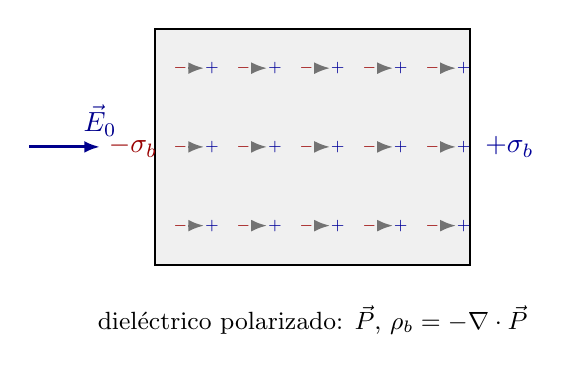
\begin{tikzpicture}[line width=0.8pt,>={Latex[length=2mm]}]
  \draw[thick,fill=black!6] (0,0) rectangle (4,3);
  % dipolos alineados
  \foreach \x in {0.6,1.4,2.2,3.0,3.8} \foreach \y in {0.5,1.5,2.5}{
    \node[red!60!black] at (\x-0.28,\y){\tiny$-$};
    \node[blue!60!black] at (\x+0.12,\y){\tiny$+$};
    \draw[->,black!55] (\x-0.18,\y)--(\x+0.02,\y);
  }
  % cargas ligadas en caras
  \node[red!60!black] at (-0.28,1.5){$-\sigma_b$};
  \node[blue!60!black] at (4.5,1.5){$+\sigma_b$};
  % campo externo
  \draw[->,blue!55!black,line width=1.1pt] (-1.6,1.5)--(-0.7,1.5) node[above]{$\vec E_0$};
  \node at (2,-0.7){\small dieléctrico polarizado: $\vec P$, $\rho_b=-\nabla\cdot\vec P$};
\end{tikzpicture}
\end{document}
